\documentclass[12pt,a4paper]{article}
\usepackage{../HBSuerDemir}

\begin{document}
\hPage{b1p2/496}
	\paragraph{}  
	    Under all these restrictions on distance and density, the \\
	    solution of a 	physical problem by 	a definite integral gives cer-\\
	    tain difficulties which can be eliminated by carefullness.
	\paragraph{} 
	    These are the reasons why the subject is treated usually \\
	    in the simpler way by multiple integrals.\\ \\
	\textbf{MOMENTS:}  
		\paragraph{} 
		    The moment of a particle P(m) of mass m located at P\\
	    	with respect to a point 0 (or a line $\ell$ , or a plane $\pi$) is the\\
	    	product of m and its distance from 0 (or $\ell$ , or $pi$). $$ M_0 = m |P0|,  M_\ell = m|P\ell|, M_\pi = m|P\pi| $$ where $|P0|, |P\ell|, |P\pi|$ denote distances of P from 0, $\ell$, $\pi$ \\respectively.\\ \\
	
	    \begin{enumerate}
	        \item [a)]\textbf{ \underline{Moment and center of an arc with mass:}}\\ 
	  Let $$y=f(x)\varepsilon(a, b)   or   x=g(y)\varepsilon D(c, d) $$ be an arc charged with density$\int (=dm/ds )$.  Then the moments of\\
	   the element of arc ds with density $\delta$ with respect to x- and\\
	 y-axis being $$d M_{0X}=y dm = y \delta ds, \hspace{20pt}  d M_{0Y} = x dm = x\delta ds,$$ $$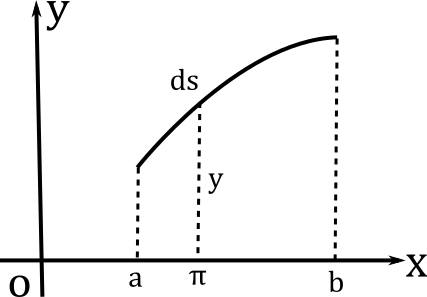
\includegraphics[width=200pt]{images/graphic1.png}$$ we have, as moments arc
	       \end{enumerate}
\end{document}